%==========================================================================

\documentclass[12pt,a4paper]{article}
\usepackage{nopageno}

%==========================================================================

%Modelo de página do IEEE
    \usepackage[lmargin=3cm,tmargin=3.5cm,rmargin=2cm,bmargin=3.5cm]{geometry}
    \usepackage[a4paper]{geometry}
    \usepackage{graphicx,eso-pic}
    
    \AddToShipoutPictureBG{%
      \AtPageUpperCenter{%
     
\includegraphics[width=\paperwidth]{Modelo21Orion.png}
      }%
    }

%-------------------------------------------------------------------------------------------------

%Pacotes de escrita:
\usepackage[utf8]{inputenc} %Pacote para acentuação
\usepackage[portuguese,brazilian]{babel} %Escrever em português brasileiro
\usepackage[T1]{fontenc} %Ajusta o texto que vem de outras fontes
\usepackage{url} %permite colocar url no texto
\usepackage[T1]{fontenc} %Ajusta o texto que vem de outras fontes
\usepackage{setspace}

%Pacotes de matemática:
	\usepackage{amsmath,amsthm,amsfonts,amssymb,dsfont,mathtools,blindtext}
	
%Pacotes usados em "Valores no gráfico:"
    \usepackage{stix} %símbolos
    \usepackage{xcolor} %cores	

%Pacote pra imagem ficar no lugar indicado no código
\usepackage{float}

%--------------------------------------------------------------------------

\begin{document}

%Modificações nos pacotes
\urlstyle{same} %ajusta a fonte do url pra ser igual à do texto
\onehalfspacing %espaçamento de 1.5 entre linhas

%==========================================================================

%CAPA
\begin{titlepage}
    \begin{center}
        \textbf{IEEE AESS RAS ORION SATELLITE SYSTEMS}\\ [0.2cm]
        \textbf{DIVISÃO DE DETERMINAÇÃO DE ATITUDE E CONTROLE}\\ [2.5cm]
        DAVID OLIVEIRA\\ [0.2cm]
        LEONARDO SIMÕES\\ [4cm]
        \textbf{RELATÓRIO SOBRE TRANSFORMAÇÃO DE COORDENADAS, COSSENOS DIRETORES E MATRIZES DE TRANSFORMAÇÃO}\\ [10.5cm]
        SANTO ANDRÉ\\ [0.2cm]
        2021\\ [0.2cm]
    \end{center}
\end{titlepage}

%==========================================================================

\section{Transformação de coordenadas}

\subsection{Grandezas escalares}

Grandezas escalares geralmente não dependem do sistema de referências. Se considerarmos que uma massa M depende das coordenadas $(x_1, x_2)$, mesmo se transformarmos o sistema de coordenadas, o seu valor se mantém $M(x_1,x_2)$ = $M(x’_1,x’_2)$. São exemplos de grandezas escalares a massa, energia e temperatura.

%--------------------------------------------------------------------------

\begin{figure}[H]
    \centering
    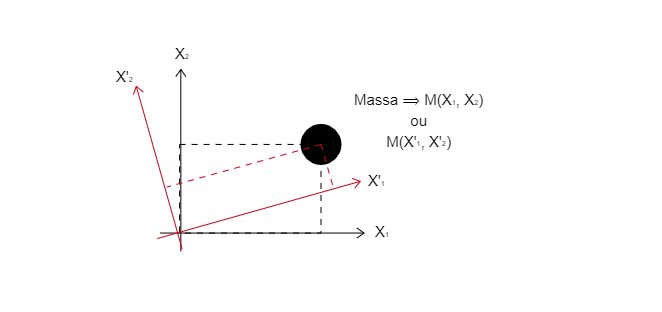
\includegraphics[width=18cm]{escalar.png} %insere a figura no texto
    \caption{Gráficos de grandezas escalares sobrepostos}
    \label{Fig01} %permite marcar a imagem
\end{figure}

%--------------------------------------------------------------------------

\subsection{Cossenos diretores}

Agora vamos entender o que são exatamente as transformações de coordenadas. Considerando o ponto $M$, ele pode ser escrito em função de suas coordenadas $(x_1,x_2)$, porém, em algumas ocasiões, é conveniente, ou, até mesmo, necessário mudar essas coordenadas. Vamos fazer uma espécie de rotação nos eixos do gráfico sem retirar o ponto do lugar - alterando os seus eixos para $(x’_1,x’_2)$ - e relacionaremos as coordenadas de um sistema com o de outro.

Através de alguns conceitos de semelhança de triângulos e trigonometria conseguiremos identificar as novas coordenadas. O objetivo é relacionar as coordenadas $(x_1,x_2)$ com $(x’_1,x’_2)$.

%--------------------------------------------------------------------------

\begin{figure}[H]
    \centering
    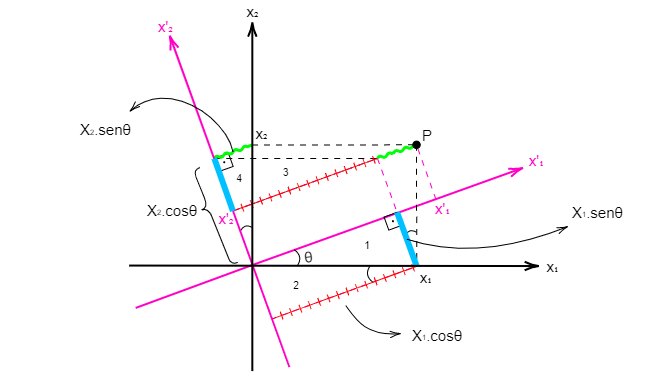
\includegraphics[width=16.5cm]{rotacao.png} %insere a figura no texto
    \caption{Rotação do eixo}
    \label{Fig01} %permite marcar a imagem
\end{figure}

%--------------------------------------------------------------------------

Por semelhança de triângulos podemos verificar que as linhas com a mesma cor são do mesmo tamanho. A linha azul no triângulo 1 tem o valor de $x_1 \cdot sen\theta$, já que é o cateto oposto ao ângulo $\theta$, e, logo, é igual ao $sen\theta$ multiplicado pela hipotenusa $x_1$. A linha verde no triângulo 4 pode ser definida a partir do mesmo raciocínio: a hipotenusa do triângulo está na vertical e o seu valor é a coordenada $x_2$, então o cateto oposto/lado verde será $x_2 \cdot sen\theta$.

Agora, para encontrar as coordenadas no sistema rotacionado, podemos ver que $x’_1$ é igual à linha vermelha pontilhada somada à linha verde, e que isso é igual ao cateto adjacente do triângulo 2, enquanto a verde é o cateto oposto ao ângulo $\theta$ do triângulo 4, e com o valor: $x_2 \cdot sen\theta$. O $x’_2$ é igual ao cateto adjacente do triângulo 4 menos a linha azul, que é $x_1 \cdot sen\theta$.\\

Então temos:

%--------------------------------------------------------------------------

\renewcommand{\labelitemii}{$\square$} %quadrado vazio item 2

\begin{enumerate}

%--------------------------------------------------------------------------

    \item Valores de $x$ e $x'$
    
        \begin{itemize}
            \item $x'_1 = x_1 \cdot cos\theta + x_2 \cdot sen\theta$
            \item $x'_2 = x_2 \cdot cos\theta - x_1 \cdot sen\theta$\\
            ou, se reescrevermos com valores em função apenas dos cossenos:
            \item  \hspace{0.1cm} $x'_1 = x_1 \cdot cos\theta + x_2 \cdot cos(\dfrac{\pi}{2} - \theta)$
            \item \hspace{0.1cm} $x'_2 = x_2 \cdot cos\theta + x_1 \cdot cos(\dfrac{\pi}{2} + \theta)$
        \end{itemize}

%--------------------------------------------------------------------------

    
    \item Cossenos diretores\\\\
    Mudando a notação:\\
    Notação 1: o ângulo entre os eixos $x_j$ e $x’_i$ é denotado por $(x’_i,x_j)$.\\
    Notação 2: definimos $\lambda_{ij}$ como o valor do cosseno do ângulo entre os eixos.

        
        \begin{itemize}
        
            \item $\lambda_{ij}=cos(x'_i,x_j)$
            
                \begin{itemize}
                    \item $\lambda_{11} = cos\theta$
                    \item $\lambda_{12} = cos(\dfrac{\pi}{2} - \theta) = sen\theta$
                    \item $\lambda_{21} = cos(\dfrac{\pi}{2} + \theta) = - sen\theta$
                    \item $\lambda_{22} = cos\theta$
                \end{itemize}
                
        \end{itemize}
        
%--------------------------------------------------------------------------
        
        Os valores $\lambda_{ij}$ são chamados de cossenos diretores. Com eles podemos relacionar quaisquer conjuntos de eixos de coordenadas. Assim, já que conseguimos encontrar eles e a sua relação entre os sistemas, podemos descobrir as coordenadas de um ponto em qualquer sistema.\\
        
        Podemos, então, escrever generalizando:
            
%--------------------------------------------------------------------------

        \begin{itemize}
            \item $x'_1 = \lambda_{11} x_1 + \lambda_{12} x_2 + \lambda_{13} x_3$
            \item $x'_2 = \lambda_{21} x_1 + \lambda_{22} x_2 + \lambda_{23} x_3$
            \item $x'_3 = \lambda_{31} x_1 + \lambda_{32} x_2 + \lambda_{33} x_3$
        \end{itemize}
        
        \begin{itemize}
            \item $x_1 = \lambda_{11} x'_1 + \lambda_{21} x'_2 + \lambda_{31} x'_3$
            \item $x_2 = \lambda_{12} x'_1 + \lambda_{22} x'_2 + \lambda_{32} x'_3$
            \item $x_3 = \lambda_{13} x'_1 + \lambda_{23} x'_2 + \lambda_{33} x'_3$
        \end{itemize}

        De forma simplificada:

        \begin{itemize}
            \item $x'_i = \sum_{j=1}^3 \lambda_{ij} x_j $
            \item $x_i = \sum_{j=1}^3 \lambda_{ji} x'_j $
        \end{itemize}
        
        
        Ao reunir esses cossenos diretores em forma de matriz, criamos a "Matriz de Transformação" ou "Matriz de Rotação", como comentada no início. Essa matriz especifica as propriedades de transformação das coordenadas de um ponto.


        \begin{itemize}
            \item  
            $ 
            \Lambda =
            \begin{pmatrix}
                \lambda_{11} & \lambda_{12} & \lambda_{13}\\ 
                \lambda_{21} & \lambda_{22} & \lambda_{23}\\
                \lambda_{31} & \lambda_{32} & \lambda_{33}
            \end{pmatrix}
            $ 
        \end{itemize}
        
        Transformações de coordenadas são como funções que levam um valor $X$ para um valor $Y$, porém que, ao invés de convertê-los em pontos, convertem vetores. A rotação é uma dessas transformações, e elas são feitas a partir de multiplicação de matrizes, sendo a matriz de cossenos usada nesse caso. Se por exemplo, fixarmos o $x_3$, a matriz ficará da seguinte forma:\\

%--------------------------------------------------------------------------

        \begin{itemize}
            \item  
            $ 
            \Lambda =
            \begin{pmatrix}
                cos\theta & sen\theta & 0\\ 
                -sen\theta & cos\theta & 0\\
                0 & 0 & 1
            \end{pmatrix}
            $ 
        \end{itemize}

%--------------------------------------------------------------------------

\end{enumerate}

%==========================================================================

%BIBLIOGRAFIA

\begin{thebibliography}{99}
     
    \bibitem{comandoslatex}
        \textit {Comandos no LaTeX}.
        Disponível em: \url{https://pt.overleaf.com/learn/latex}.
           
    \bibitem{mathcha}
        ERLAN, José. 
        \textit {Mathcha - Áreas Hachuradas}.
        Disponível em: \url{https://www.youtube.com/watch?v=e7XWs3U_jug&ab_channel=Matem%C3%A1ticacomProf.Jos%C3%A9Erlan},
        2020.
        
    \bibitem{capalatex}
        FERNANDO, Luiz. 
        \textit {Primeiros passos LATEX - Capa para trabalho}.
        Disponível em: \url{http://www-mat-ams.blogspot.com/2013/05/primeiros-passoslatex-capa-para-trabalho}.html,
        2013.
      
    \bibitem{bibliografia2latex}
        \textit {How to change the font of URL in the bibliography [duplicate]}.
        Disponível em: \url{https://tex.stackexchange.com/questions/106622/how-to-change-the-font-of-url-in-the-bibliography}.

    \bibitem{bibliografialatex}
        \textit {LaTeX/Bibliography Management}.
        Disponível em: \url{https://en.wikibooks.org/wiki/LaTeX/Bibliography_Management}.
        
    \bibitem{hyperlinkslatex}
        \textit {LaTeX/Hyperlinks}.
        Disponível em: \url{https://en.wikibooks.org/wiki/LaTeX/Hyperlinks}.
              
    \bibitem{esopic}
        NIEPRASCHK, Rolf.
        \textit {The eso-pic package}.
        Disponível em: \url{https://cs.brown.edu/about/system/software/latex/doc/eso-pic.pdf},
        2002.
        
    \bibitem{cursolatex}
        SILVA, Jaqueline. 
        \textit {Curso de introdução ao LaTeX}.
        Disponível em: \url{https://youtube.com/playlist?list=PLb735fZHArLaD_RFIiNQx7_WHSnhdy60e},
        2020.

    \bibitem{cossenosdiretores}
        SOUZA, Leonardo. 
        \textit {Transformação de coordenadas, cossenos diretores, matriz de transformação}.
        Disponível em: \url{https://www.youtube.com/watch?v=mdvItbnnVbw&ab_channel=LeonardoSouza},
        2021.

\end{thebibliography}

%==========================================================================

\end{document}